\documentclass[conference]{IEEEtran}
\usepackage{times}
\usepackage{amsmath}
\usepackage[disable]{todonotes}
\usepackage{algorithm}
\usepackage[noend]{algpseudocode}
\usepackage{graphicx}
\makeatletter
\def\BState{\State\hskip-\ALG@thistlm}
\makeatother
\newcommand\nameeq[2]{\phantom{\text{#2}}&&#1&&\text{#2}}
\newtheorem{theorem}{Theorem}

% numbers option provides compact numerical references in the text. 
\usepackage[numbers]{natbib}
\usepackage{multicol}
\usepackage[bookmarks=true]{hyperref}

\pdfinfo{
   /Author (Gaurav Mahajan)
   /Title  (Notes)
   /CreationDate (\today)
   /Subject (NN)
   /Keywords (local;minima)
}

\begin{document}

% paper title
\title{Local Minima 2,1,2}

% You will get a Paper-ID when submitting a pdf file to the conference system
%\author{Author Names Omitted for Anonymous Review. Paper-ID [add your ID here]}

%\author{\authorblockN{Michael Shell}
%\authorblockA{School of Electrical and\\Computer Engineering\\
%Georgia Institute of Technology\\
%Atlanta, Georgia 30332--0250\\
%Email: mshell@ece.gatech.edu}
%\and
%\authorblockN{Homer Simpson}
%\authorblockA{Twentieth Century Fox\\
%Springfield, USA\\
%Email: homer@thesimpsons.com}
%\and
%\authorblockN{James Kirk\\ and Montgomery Scott}
%\authorblockA{Starfleet Academy\\
%San Francisco, California 96678-2391\\
%Telephone: (800) 555--1212\\
%Fax: (888) 555--1212}}


% avoiding spaces at the end of the author lines is not a problem with
% conference papers because we don't use \thanks or \IEEEmembership


% for over three affiliations, or if they all won't fit within the width
% of the page, use this alternative format:
% 
%\author{\authorblockN{Michael Shell\authorrefmark{1},
%Homer Simpson\authorrefmark{2},
%James Kirk\authorrefmark{3}, 
%Montgomery Scott\authorrefmark{3} and
%Eldon Tyrell\authorrefmark{4}}
%\authorblockA{\authorrefmark{1}School of Electrical and Computer Engineering\\
%Georgia Institute of Technology,
%Atlanta, Georgia 30332--0250\\ Email: mshell@ece.gatech.edu}
%\authorblockA{\authorrefmark{2}Twentieth Century Fox, Springfield, USA\\
%Email: homer@thesimpsons.com}
%\authorblockA{\authorrefmark{3}Starfleet Academy, San Francisco, California 96678-2391\\
%Telephone: (800) 555--1212, Fax: (888) 555--1212}
%\authorblockA{\authorrefmark{4}Tyrell Inc., 123 Replicant Street, Los Angeles, California 90210--4321}}


\maketitle

\begin{abstract}
Trying to find out if there are some interesting local minimas in 2,1,2 neural network. 2 inputs, 1 hidden relu, 2 outputs.
\end{abstract}

\IEEEpeerreviewmaketitle

\section{Introduction}
We assume throughout the discussion that inputs are positive, so $x > 0$.
It is clear that linear nns do not have local minima. The next obvious step is to investigate non linear relu nns.
Looking at 1,1,1, it is clear that there is no local minima, it behaves like linear until $a00 > 0$ and outputs $0$ otherwise.

\begin{figure}
	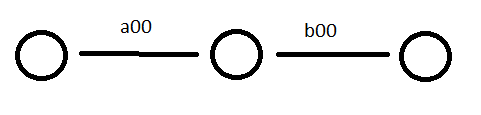
\includegraphics[width=\linewidth]{images/nn/111.png}
	\caption{1,1,1 NN}
	\label{fig:111}
\end{figure}

Two directions forward:
\begin{itemize}
	\item Increase the number of hidden neurons
	\item Increase the number of inputs
\end{itemize}

\section{1,n,1: On increasing the size of hidden neurons} 

\begin{figure}
	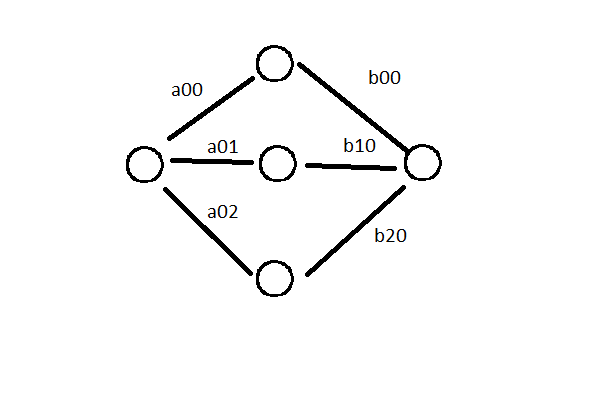
\includegraphics[width=\linewidth]{images/nn/131.png}
	\caption{1,3,1 NN}
	\label{fig:131}
\end{figure}

Intuitively, when all weights are positive or negative, this behaves like a linear netowrk or always zero. The case that is to be investigated is when some $a0i > 0$ while some $a0j < 0$. The major observation which distinguishes 1 input from multiple inputs is that these neurons will behave exactly the same for each example xi in 1,n,1.

So, if neuron n is off for example xi, it will be turned off for example xj because all examples are positive which implies any neuron only turns off when corresponding a < 0. Now, because of this,when any neuron is turned off, 1,n,1 behaves like 1,n-1,1 in that "region". The set where any neuron is off is actually a connected region (this is true for any n,n,n network, but in this case it is actually half of the space i.e $a < 0$). Now, local in these regions there can not be any local minima because they all behave linearly inductively. The only case which needs to be checked is that global minimas for these regions can be actually local minima to the entire space. This is equivalent to saying "Does 1,n,1 make an improvement on the loss over 1,n-1,1?". 1,n,1 actually contains all the global/local minimas of 1,n-1,1 and the only way it can create new local minimas is if it comes up with a better global minima on input examples.


\section{2,1,2: Increasing the number of inputs}

\begin{figure}
	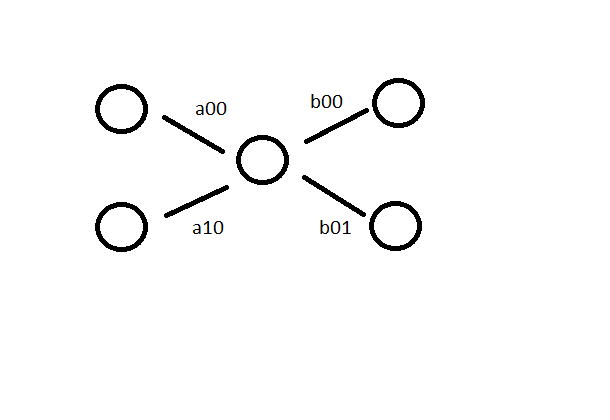
\includegraphics[width=\linewidth]{images/nn/212.png}
	\caption{2,1,2 NN}
	\label{fig:212}
\end{figure}

1,1,1 does not have a local minima. Increasing the number of inputs immediately lead to a local minima. The simplest case 2,1,2 has a family of minimas.

Denote by ri the output of relu unit on example xi. Then, we can easily see

\begin{align}
ri = 0 &\iff a00*xi0 < -(xi1*a10) \\
r0 = 0 &\iff a00*x00 < -(x01*a10) \\
r1 = 0 &\iff a00*x10 < -(x11*a10)
\end{align}

Equation 1 and 2 are lines in (a00,a01) plane. This leads to four regions. For input (1,0) and (1,1), the lines are (with a00 as x and a01 as y)
\begin{align}
r0 = 0 &\iff x < 0 \\
r1 = 0 &\iff x < -y
\end{align}

\begin{figure}
	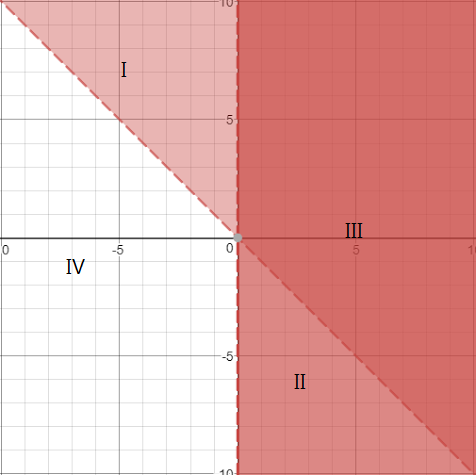
\includegraphics[width=\linewidth]{images/nn/212loss.png}
	\caption{2,1,2 Loss NN}
	\label{fig:212loss}
\end{figure}

Region I ($x<0$ and $x>-y$) has neuron working only for example x1, region II ($x>0$ and $x<-y$) has neuron working only for example x0, region III ($x>0$ and $x>-y$) has the neuron working for both examples and region IV has neuron turned off for both examples.

Loss in Region I will always have a non zero component from example x0, so the minimum loss there will be $>= norm(y0)$.
In fact (given b00,b01), the output from the neuron for example x1 which leads to minima is unique, let it be r(for x0, it will be 0). 

\begin{align}
a00*x10 + x11*a10 &= r
\end{align} 

This is an equation of a line. a00 and a01 which satisfy this equation and lie in region I are local minimas (again, given b00,b01, changing the b00,b01 will give another line of local minimas, the loss on all such lines is same.)

\begin{figure}
	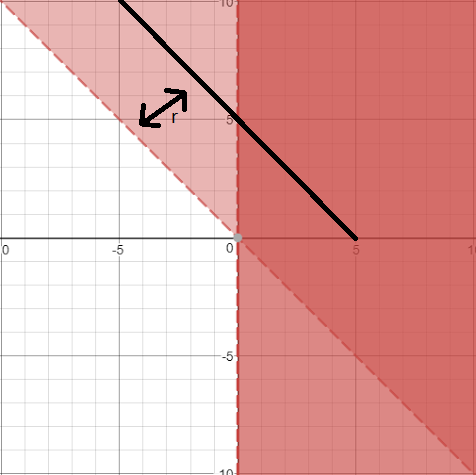
\includegraphics[width=\linewidth]{images/nn/212r.png}
	\caption{2,1,2 local minima}
	\label{fig:212localminima}
\end{figure}

The natural question is would gradient descent fall in these local minimas. If you start from region I, would always lead to these minimas? Would starting from region III, safeguard convergence to global minima?


\section*{Acknowledgments}

%% Use plainnat to work nicely with natbib. 

\bibliographystyle{plainnat}
\bibliography{references}

\end{document}


